\section{\ttt{3D} classification and Refinement}

 \begin{figure}[H]
  \centering
  \captionsetup{width=.8\linewidth} 
  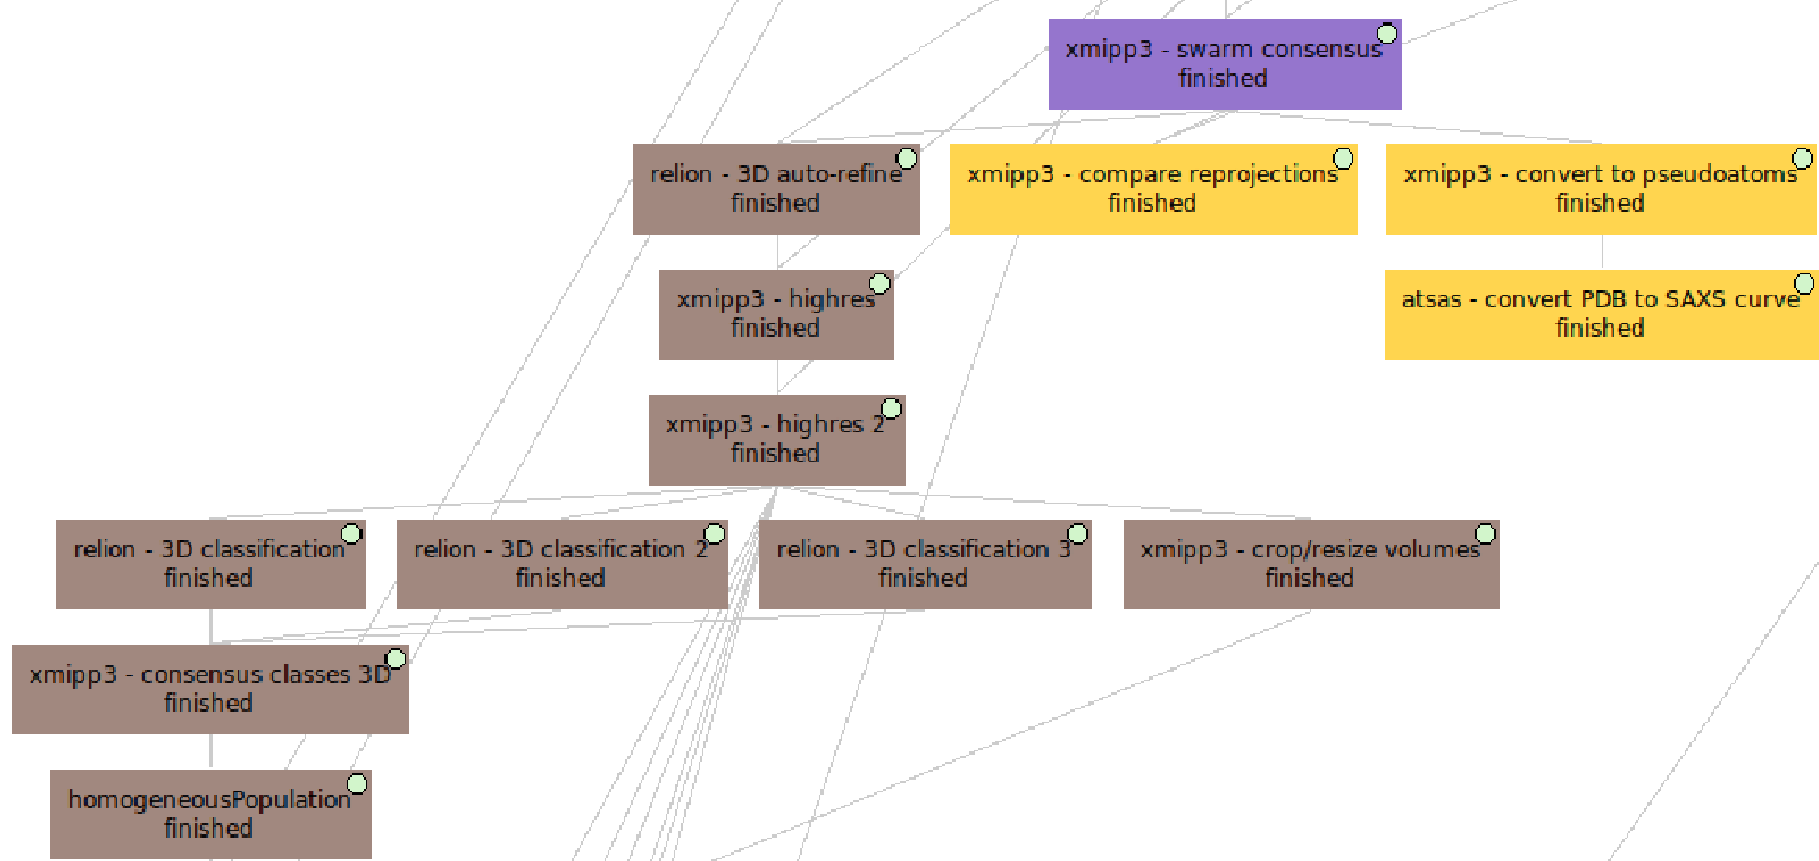
\includegraphics[width=1\textwidth]
  {{images/workflow_6.pdf}}
  \caption{Refinement and \ttt{3D} classification (Brown color).}
  \label{fig:workflow_6}
  \end{figure}

\ttt{3D} classification and Refinement are the two last overlapping steps in image processing. They consume the most time and resources with the aim of obtaining a \ttt{3D} map at the highest possible resolution. This is only feasible if data are homogeneous enough, $i.e.$, if data represent a unique conformation of the specimen.\\

Before starting with the \ttt{3D} classification properly, three consecutive steps of refinement will be performed with our initial map. The first approach to get a high resolution map in a fully automated manner was performed with the algorithm $Relion$ \ttt{auto\_refine}, based on an empirical Bayesian approach. This procedure employs the so-called gold-standard Fourier Shell Correlation (FSC) to estimate the resolution. Combined with a novel procedure to estimate the accuracy of the angular assignments, the algorithm converges. We have implemented it in the protocol \scommand{relion- \ttt{3D} auto-refine} (\ffigure{fig:initial_vol_1}). In the \ttt{Input} tap of this protocol form we include the subset of homogeneous particles  selected previously. The initial volume will be included in the \ttt{Reference 3D map} tap, as well as a \ttt{Initial low pass-filter (A)} of 60.0. This tap gives you the possibility of using \ttt{Reference mask (optional)} and, in some cases, $e.g$ non-empty icosahedral viruses, a \ttt{Second reference mask (optional)}.

\begin{figure}[H]
  \centering
  \captionsetup{width=.8\linewidth} 
  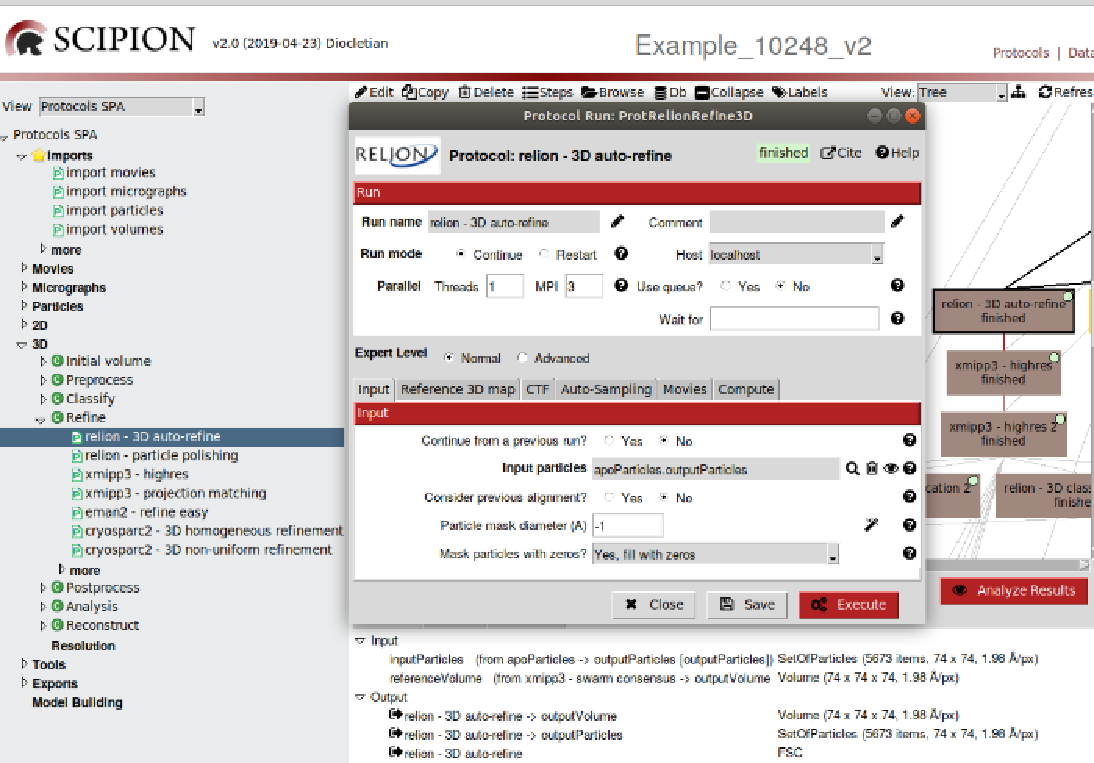
\includegraphics[width=0.95\textwidth]
  {{images/relion_3D_auto_refine_1.pdf}}
  \caption{Completing the params of the protocol \scommand{relion- \ttt{3D} auto-refine}.}
  \label{fig:relion_3D_auto_refine_1}
  \end{figure}

There are three questions in the tab \ttt{CTF}: 
\begin{itemize}
 \item \ttt{Do CTF correction?}, set to \ttt{Yes} to perform full phase + amplitude CTF correction.
 \item \ttt{Has reference been CTF-corrected?}, set to \ttt{No} because the Fourier transforms of the reference projections are not multiplied by the \ttt{CTF} in the first iteration. 
 \item \ttt{Do manual grouping ctfs?}, set to \ttt{No} because we have enough number of particles that we do not need to group them.
\end{itemize}

The \ttt{Angular sampling interval (deg)} option in the tab \ttt{Auto-Sampling} will be used only in the first few iterations. Later the algorithm will automatically increase its value until convergence. For symmetries lower than octahedral or icosahedral we use the default values of \ttt{Angular sampling interval (deg)} and \ttt{Local search from auto-sampling (deg)}.\\

\ttt{Movies} tab allows to align movie-particles of each frame and execute later a protocol of particle polishing.\\

After executing 7 iterations a refined map of 5.05 \AA\ of final resolution was obtained as output, with the same size and sampling rate that we had in the inputs. Press \scommand{Analyze Results} and visualize any iteration or the last one by default. Concerning particles, their angular assignment and the \ttt{\*\_optimiser.star file}, with general information about the refinement process, can be shown. Different volumes can be \ttt{2D} or \ttt{3D} visualized, such as each half map, both, or the final one. \ttt{SSRN} and resolution \ttt{FSC} plots are also available.\\

The next two following steps of refinement have been performed with the $Xmipp$ algorithm \ttt{highres} \citep{sorzano2018new} that we have implemented in the protocol \scommand{xmipp3-highres} (\ffigure{fig:xmipp_highres_1}). This method computes a weight for each particle and performs both global and local alignment. Iterations can be performed one by one, removing particles that worse fit the map from one iteration to the next one. This \ttt{3D} refinement protocol uses as input the refined map obtained from $Relion$ \ttt{auto\_refine} and the same set of particles used by this algorithm. The \ttt{Symmetry group} has been also included in the \ttt{Input} tap. In the \ttt{Angular assignment} tap we choose \ttt{Global} as \ttt{Image alignment} and 1 \ttt{Number of iterations} with 4 \AA\ as \ttt{Max. Target Resolution}.

\begin{figure}[H]
  \centering
  \captionsetup{width=.8\linewidth} 
  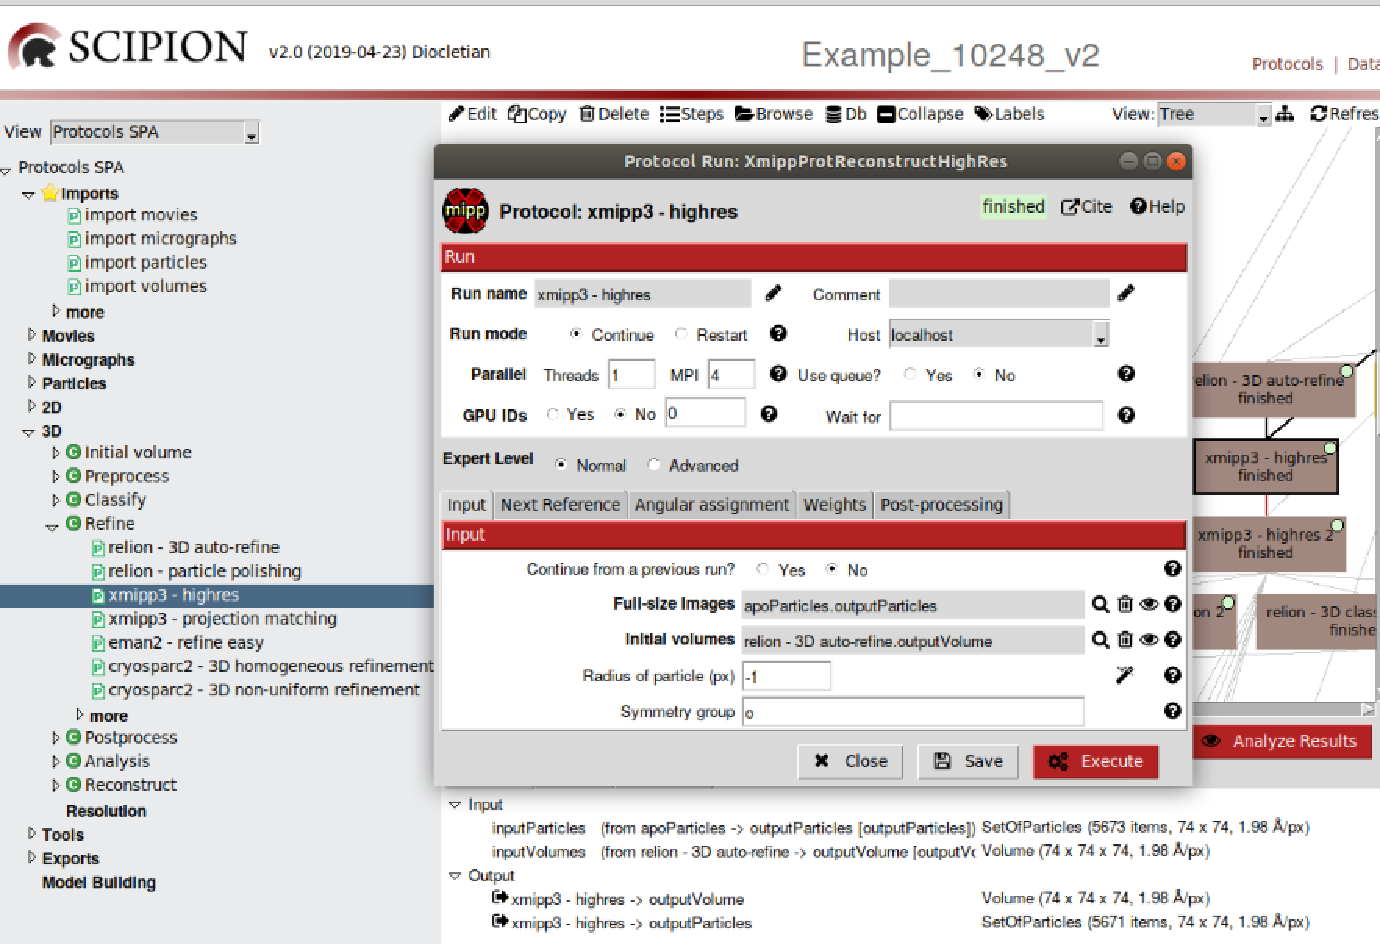
\includegraphics[width=0.95\textwidth]
  {{images/xmipp_highres_1.pdf}}
  \caption{Filling in the params of the protocol \scommand{xmipp3-highres}.}
  \label{fig:xmipp_highres_1}
  \end{figure}

This protocol also generates one map as output with the initial size and sampling rate. Press \scommand{Analyze Results} to check the results of the iteration 1. Particles and map can also visualized. 2 particles have been rejected.\\

The second time that we execute the protocol \scommand{xmipp3-highres} we select the map obtained in the previous step and the same set of particles as input. In the tap \ttt{Angular assignment} we replace \ttt{Global} by \ttt{Local} in the \ttt{Image alignment} param. The rest of the params remain unchanged since we have selected \ttt{Yes} in the param \ttt{Continue from a previous run?} of tap \ttt{Input}. In this case, another map has been generated as output with the same size and sampling rate. 6 particles have been discarded this time.\\

To continue with the refinement process and to obtain a better resolution, we are to start executing three times the same algorithm of $Relion$ \ttt{3D classification} that we have implemented in the protocol \scommand{relion-3D classification} (\ffigure{fig:relion_3Dclassification}). In the tap \ttt{Input} we include the particles derived from executing the previous protocol \scommand{xmipp3-highres}. The map derived from this protocol will be the \ttt{Input volume(s)} in the tap \ttt{Reference 3D map}. The optimization params appear in the tap \ttt{Optimization}: 3 \ttt{Number of classes} and 25 \ttt{Number of iterations}. As \ttt{Regularisation parameter T} values 3-4 are common for \ttt{3D} classificacion.

\begin{figure}[H]
  \centering
  \captionsetup{width=.8\linewidth} 
  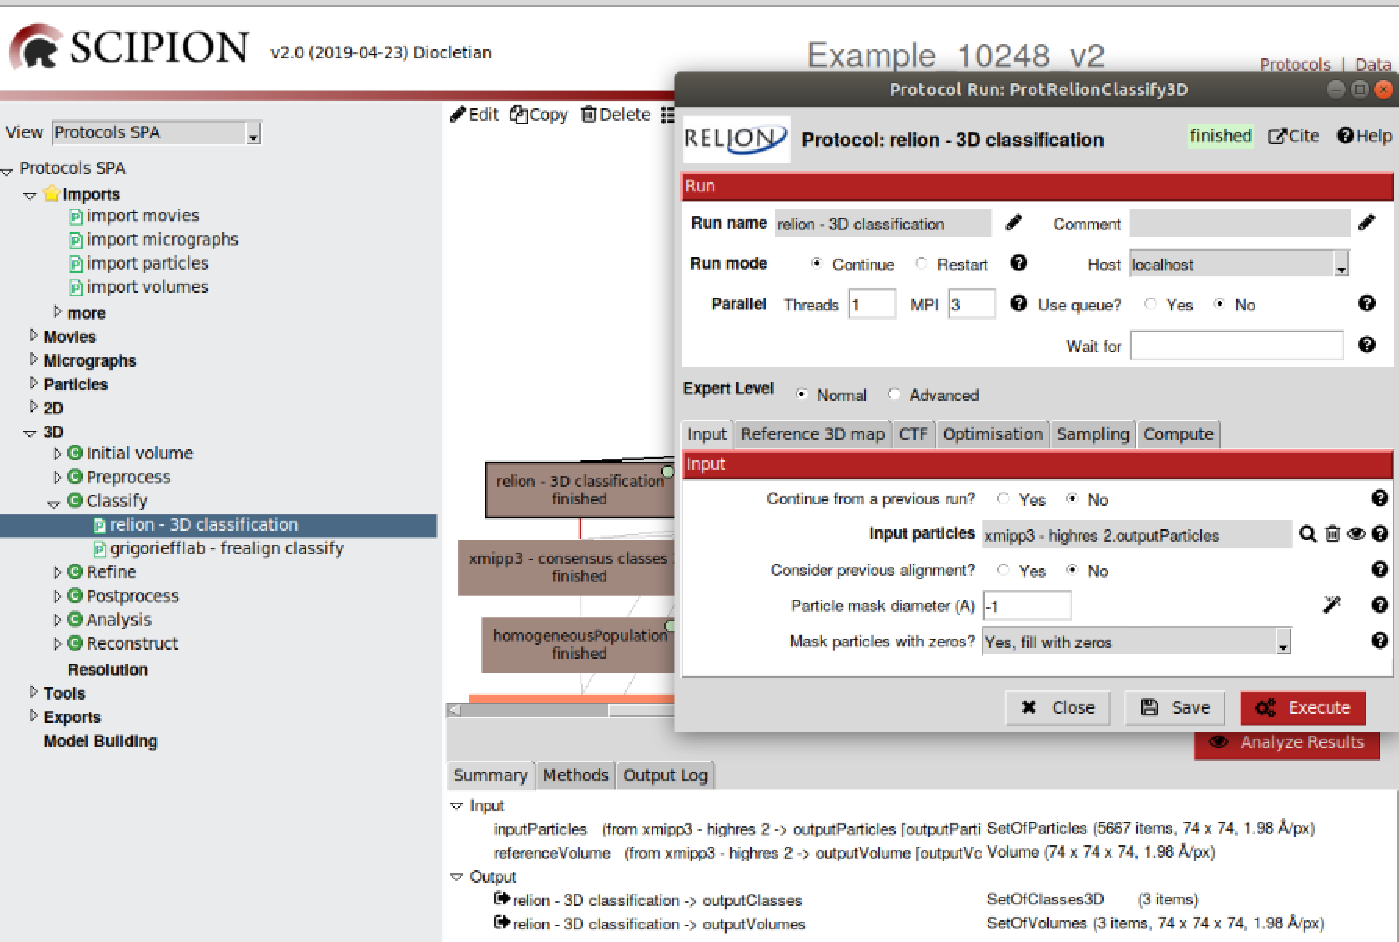
\includegraphics[width=0.95\textwidth]
  {{images/relion_3Dclassification.pdf}}
  \caption{Completing the params of the protocol \scommand{relion-3D classification}.}
  \label{fig:relion_3Dclassification}
  \end{figure}
  
The output of these three protocols are 3 maps 
       
